\chapter{Optical MIMO: Exploring the color dimension}
\label{chapter:mimoColor}
\thispagestyle{myheadings}
As seen in previous chapter, imaging receivers have the potential to to provide significant performance gains for a spatial MIMO OWC system. To incorporate these in portable devices, they must address challenges of being low powered, have fast sampling rates while incorporating optics, sensor and electronics in a small form factor.

This chapter explores the color dimension to establish an optical MIMO channel. It investigates color shift keying (CSK) as specified in IEEE 80.15.7 standard PHY  \rmnum{3}. The standard specifies a simplified linear system model for CSK. The human visual perception model is non--linear and needs to be considered while providing illumination. Thus a non--linear CSK model is investigated for different color band combinations. Luminous-signal-to-noise ratio metric is introduced to make fair performance comparisons between different modulation techniques operating at different average radiant flux, but same average luminous flux levels. Metameric modulation then further explores color dimension by using multiple sets of LEDs to transmit information over metamerically equivalent SPDs \cite{but12a}.

% -------------------------------------
% SECTION: IEEE 802.15.7
% -------------------------------------
\section{IEEE 802.15.7 - PHY \rmnum{3}}
\label{sec:ieeestd}
\graphicspath{{_MIMOColor/figures_csk/}}
LED based luminaires are energy efficient and are thus being widely adopted in indoor spaces to provide illumination. In order to dynamically control the rendered illumination spectrum, luminaires contain multiple elements of at least three colors of LEDs. Different SPDs can be rendered by mixing different ratios of radiant flux emitted from the multiple LEDs comprising a luminaire. Each resulting SPD realizes a different color mix to the human eye.

Any SPD within the visible range of electromagnetic spectrum can produce a stimulus when incident on the sensors of the human eye (rod and cones) and has a color associated with it. This color can also be represented by its intensity, hue and saturation. While intensity is a measure of the total power comprising the SPD, hue and saturation are subjective parameters analogous to mean and spread of the wavelengths comprising the SPD and are quantified by a chromaticity coordinate. The \textit{commission internationale de l'eclairage} (CIE) has specified the CIE 1931 XYZ color space (CIE-CS) that provides a mathematical model to represent the chromaticity of radiation in the visible range as a point in a 2-dimensional plane. Let a luminaire be comprised of three types of LEDs, namely LED$_{n}$; $n\in$ \text{\{i, j, k\}}. The chromaticity of each LED can be represented by a coordinate ($x_{n}$, $y_{n}$) on the CIE-CS. When different intensities of radiant flux emitted by three types of LEDs are combined, the chromaticity coordinate of the resultant SPD will lie inside the triangle formed by coordinates of the LEDs themselves.

\renewcommand{\arraystretch}{1.1}
\begin{table}[t]
\centering
\begin{tabular}{|c|c|c|c|c|}
\hline
\multirow{2}{*}{\textbf{CB$_{u}$}} & \textbf{Band} & \textbf{Center} & \multirow{2}{*}{\textbf{x}} & \multirow{2}{*}{\textbf{y}}\\
 & \textbf{(nm)} & \textbf{(nm)} & & \\
\hline
CB$_{0}$ & 380 - 478 & 429 & 0.169 & 0.007\\
\hline
CB$_{1}$ & 478 - 540 & 509 & 0.011 & 0.733\\
\hline
CB$_{2}$ & 540 - 588 & 564 & 0.402 & 0.597\\
\hline
CB$_{3}$ & 588 - 633 & 611 & 0.669 & 0.331\\
\hline
CB$_{4}$ & 633 - 679 & 656 & 0.729 & 0.271\\
\hline
CB$_{5}$ & 679 - 726 & 703 & 0.734 & 0.265\\
\hline
CB$_{6}$ & 726 - 780 & 753 & 0.734 & 0.265\\
\hline
\multicolumn{5}{c}{ }
\end{tabular}
\caption{Color bands as outlined in IEEE 802.15.7}
\label{tCB}
\end{table}
\renewcommand{\arraystretch}{1.0}

\begin{figure}[!t]
\centering
		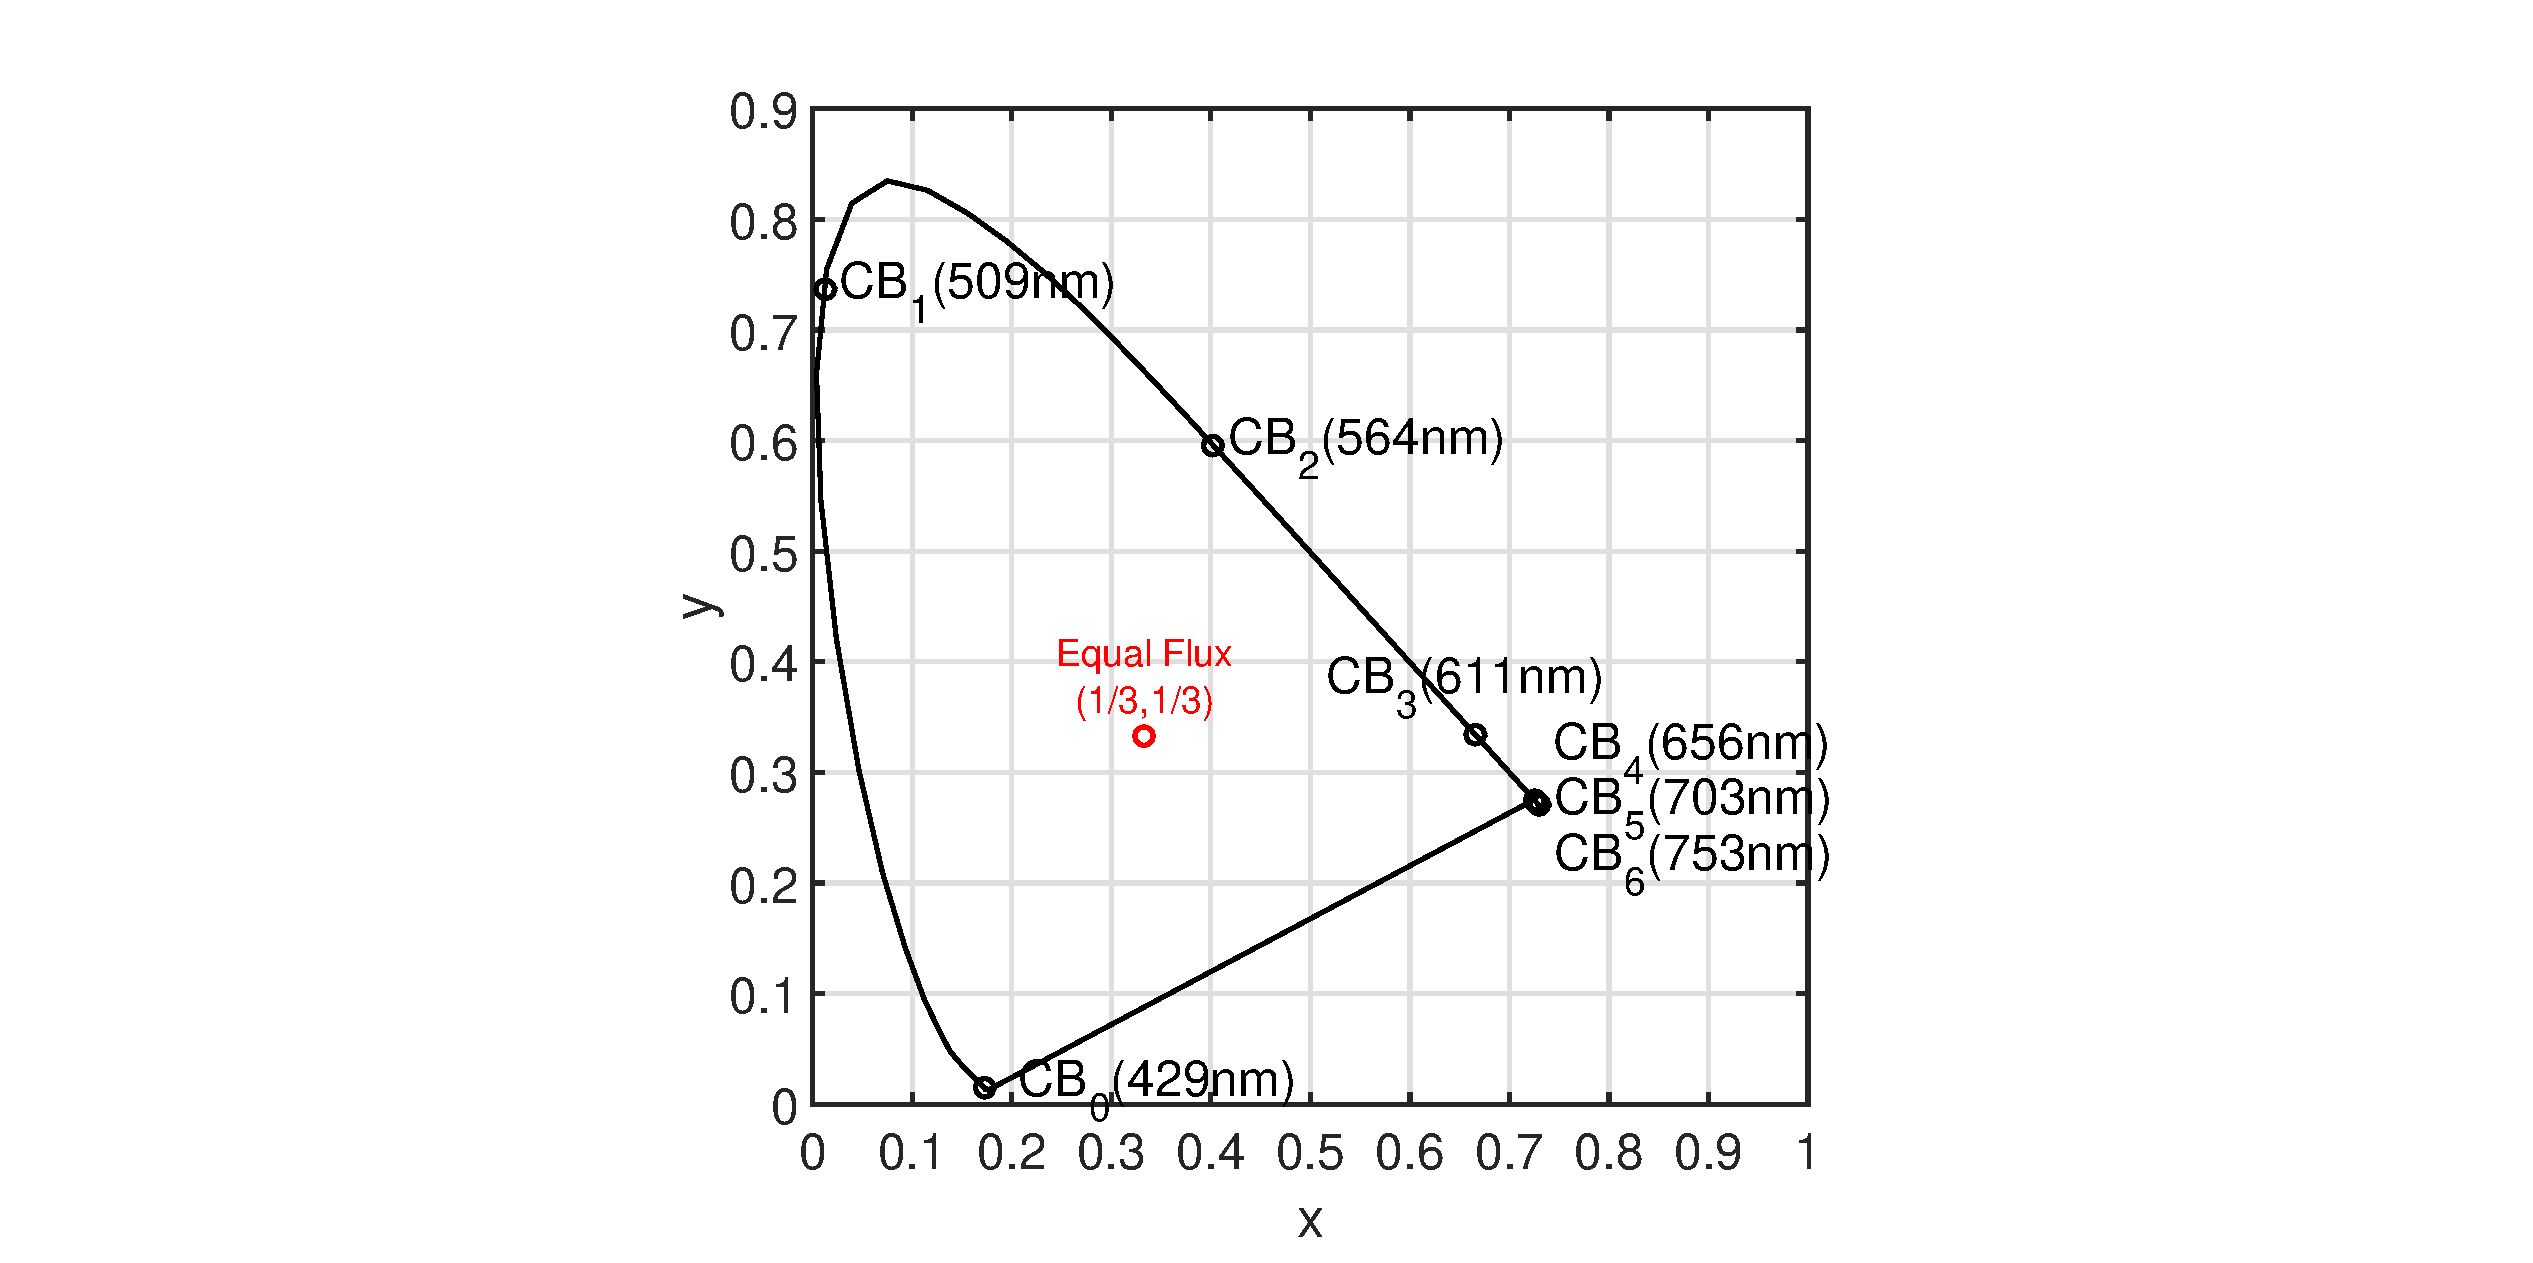
\includegraphics[trim={4.3in 0in 4.3in 0.5in}, clip=true, width=3.0in]{CBCcenters.eps}
	\caption{Color band centers on CIE-CS}
	\label{figCBCcenters}
\end{figure}


The IEEE standard for short-range OWC using visible light specifies CSK as the modulation technique of choice under the PHY \rmnum{3} specifications \cite{IEEE802.15.7}. For the rest of this chapter, the noun `standard' shall imply the IEEE 802.15.7 standard, specifically chapter 12 on PHY \rmnum{3} specifications. The standard outlines linear system configurations with $M$-ary CSK to achieve up to 96 Mb/s data rate. Reference \cite{raj12a} provides an overview of modulation and dimming techniques specified within the standard while reference \cite{sin13a} studies select color bands for CSK.

CSK is a modulation technique in which information is transmitted through changes in chromaticity coordinates. This can be achieved by varying the intensities of LED$_{n}$ over time. To select sources for CSK implementation, the standard specifies 7 different color bands - CB$_{u}$; $0\leq u < 7$ by splicing the visible spectrum range into 7 contiguous segments as shown in Table \ref{tCB}. The center wavelength of each segment as represented on CIE-CS is illustrated in \figurename{ }\ref{figCBCcenters}. Note that even though center wavelengths of CB$_{4}$, CB$_{5}$ and CB$_{6}$ are 47 nm -- 50 nm apart, the distance between their chromaticity coordinates is very small. The CIE-CS is designed such that the SPD resulting from identical flux emitted by the three primary sources maps to coordinate (1/3, 1/3) which is shown in \figurename{ }\ref{figCBCcenters}. We can define a color sector on the CIE-CS as the region enclosed by a color band on the perimeter and coordinate (1/3, 1/3). Though not explicitly mentioned in the standard, it is assumed that SPD of each LED$_{n}$ must belong to a different color sector. To study the performance of CSK independent of specific LED characteristics, it is generally assumed that the chromaticity coordinate of an LED belonging to a color sector corresponds to the center wavelength of a color band CB$_{u}$ at the perimeter of the sector as illustrated in \figurename{ }\ref{figCBCcenters}.

\renewcommand{\arraystretch}{1.1}
\begin{table}[t]
\centering
\begin{tabular}{|c|c|c|c|}
\hline
Color band combination & \multicolumn{3}{c|}{Color band '$u$' for CBC$_{v}$} \\
\cline{2-4}
\textbf{CBC$_{v}$} & \textbf{Band i} & \textbf{Band j} & \textbf{Band k} \\
\hline
CBC$_{1}$ & 6 & 2 & 0 \\
\hline
CBC$_{2}$ & 6 & 1 & 0 \\
\hline
CBC$_{3}$ & 5 & 2 & 0 \\
\hline
CBC$_{4}$ & 5 & 1 & 0 \\
\hline
CBC$_{5}$ & 4 & 2 & 0 \\
\hline
CBC$_{6}$ & 4 & 1 & 0 \\
\hline
CBC$_{7}$ & 3 & 2 & 0 \\
\hline
CBC$_{8}$ & 3 & 1 & 0 \\
\hline
CBC$_{9}$ & 2 & 1 & 0 \\
\hline
\end{tabular}
\caption{Color bands combinations as outlined in IEEE 802.15.7}
\label{tCBC}
\end{table}
\renewcommand{\arraystretch}{1.0}

\afterpage{%
\clearpage
\begin{landscape}% Landscape page
\renewcommand{\arraystretch}{1.1}
\begin{table}
\centering
\begin{tabular}{|c|c|c|c|}
\hline
\textbf{m} & \textbf{$M$ = 4} & \textbf{$M$ = 8} & \textbf{$M$ = 16} \\
\hline
0 & C$^{v}_{\text{j}}$ & (2C$_{4}$+C$_{5}$)/3 & C$^{v}_{\text{j}}$\\
1 & (C$^{v}_{\text{i}}$+C$^{v}_{\text{j}}$+C$^{v}_{\text{k}}$)/3 & (2C$_{a}$+C$_{b}$)/3; C$_{a}$=(C$_{b}$+C$_{3}$+C$_{5}$)/3; C$_{b}$=(C$_{4}$+C$_{5}$)/2 & (C$_{0}$+C$_{3}$+C$_{5}$)/3 \\
2 & C$^{v}_{\text{k}}$ & (2C$_{a}$+C$_{b}$)/3; C$_{a}$=(C$_{b}$+C$_{3}$+C$_{7}$)/3; C$_{b}$=(C$_{4}$+C$_{7}$)/2 & (C$_{3}$+C$_{6}$+C$_{10}$)/3 \\
3 & C$^{v}_{\text{i}}$ & (C$_{5}$+C$_{7}$)/2 & (2C$_{0}$+C$_{9}$)/3 \\
\cline{2-2}
4 & & C$^{v}_{\text{j}}$ & (C$_{0}$+2C$_{8}$)/3 \\
5 & & C$^{v}_{\text{k}}$ & (2C$_{0}$+C$_{8}$)/3 \\
6 & & (2C$_{4}$+C$_{7}$)/3 & (C$_{0}$+C$_{8}$+C$_{9}$)/3 \\
7 & & C$^{v}_{\text{i}}$ & (C$_{4}$+C$_{5}$+C$_{6}$)/3 \\
\cline{3-3}
8 & & & C$^{v}_{\text{i}}$ \\
9 & & & C$^{v}_{\text{k}}$ \\
10 & & & (C$_{0}$+2C$_{9}$)/3 \\
11 & & & (C$_{9}$+C$_{10}$+C$_{15}$)/3 \\
12 & & & (2C$_{8}$+C$_{9}$)/3 \\
13 & & & (C$_{4}$+C$_{8}$+C$_{12}$)/3 \\
14 & & & (C$_{6}$+C$_{12}$+C$_{15}$)/3 \\
15 & & & (C$_{8}$+2C$_{9}$)/3 \\
\hline
\end{tabular}
\caption[Design rules to compute constellation points for $M$-ary CSK]{Design rules to compute constellation points for $M$-ary CSK. Each row computes C$_{m}$, the chromaticity coordinate for m$^{th}$ codeword for any given CBC$_{v}$. C$^{v}_{n}$ is the chromaticity coordinate of color band $n\in$ \{i, j, k\} belonging to CBC$_{v}$.}
\label{tMCSK}
\end{table}
%Each row computes C$_{m}$, the chromaticity coordinate for m$^{th}$ codeword for any given CBC$_{v}$. C$^{v}_{n}$ is the chromaticity coordinate of color band $n\in$ \{i, j, k\} belonging to CBC$_{v}$.
\renewcommand{\arraystretch}{1.0}
\end{landscape}
\clearpage% Flush page
}

To implement CSK using 3 types of LEDs, the standard defines different sets of 3 color bands and calls each set a color band combination (CBC). The 3 different types of LEDs forming a CBC are ordered in a descending manner based on the center wavelength of the color band they belong to and each such band is called `band i', `band j' and `band k' respectively. 9 such CBC$_{v}$; $1\leq v\leq 9$ are defined in the standard and are outlined in Table \ref{tCBC}. The generalized notation CB$^{v}_{n}$ is used to indicate color band of type $n\in$ \text{\{i, j, k\}} belonging to CBC$_{v}$. Thus in Table \ref{tCBC}, the cell representing row for CBC$_{v}$ and column for band $n$ provides index $u$ for the color band represented by notation CB$^{v}_{n}$. Using this notation CB$^{1}_{\text{i}}$ $\equiv$ CB$_{6}$ while CB$^{2}_{\text{j}}$ $\equiv$ CB$_{1}$ and so on.

\afterpage{%
%\clearpage
%\begin{landscape}% Landscape page
\begin{figure}[!t]
	\centering
		\begin{subfigure}{\textwidth}
		\centering
			\includegraphics[trim={0.05in 0.0in 0.25in 0.2in}, clip=true, width=0.45\textwidth]{CBCrules4.eps}
			\caption{4-CSK}
			\label{fig4Const}
		\end{subfigure}
		\vfill
		\begin{subfigure}{\textwidth}
		\centering
			\includegraphics[trim={0.05in 0.0in 0.25in 0.2in}, clip=true, width=0.45\textwidth]{CBCrules8.eps}
			\caption{8-CSK}
			\label{fig8Const}
		\end{subfigure}
		\vfill
		\begin{subfigure}{\textwidth}
		\centering
			\includegraphics[trim={0.05in 0.0in 0.25in 0.2in}, clip=true, width=0.45\textwidth]{CBCrules16.eps}
			\caption{16-CSK}
			\label{fig16Const}
		\end{subfigure}
	\caption{$M$-ary CSK (normalized) constellation design rules}
	\label{figConst}
\end{figure}
%\end{landscape}
\clearpage% Flush page
}

For an $M$-ary CSK using CBC$_{v}$, the design rules to compute the $M$ different constellation points are provided in the standard and their values are outlined in \cite{cskxy}. Let C$^{v}_{n}$ $\equiv$ (x$^{v}_{n}$, y$^{v}_{n}$) be chromaticity coordinate corresponding to CB$^{v}_{n}$. Let C$_{m}$ $\equiv$ ($x_{m}$, $y_{m}$); $0\leq m <$ $M$ be chromaticity coordinate corresponding to m$^{th}$ codeword. Then Table 3 outlines the design rules for computing the constellation points. C$^{v}_{n}$ can be looked up from Table \ref{tCBC} and Table \ref{tCB}. Using these values, remaining C$_{m}$ can then be computed using rules from Table \ref{tMCSK}. Normalized constellation design rules for $M$-ary CSK are illustrated in \figurename{ }\ref{figConst}. Points I, J and K represent normalized coordinates for the $n$ color bands comprising a CBC. 

%\afterpage{%
%\clearpage
%\begin{landscape}% Landscape page
%
%\end{landscape}
%\clearpage% Flush page
%}

% -------------------------------------
% SECTION: CSK
% -------------------------------------
\section{Color Shift Keying}
\label{sec:csk}
CSK stuff goes here.

% -------------------------------------
% SECTION: Metameric Modulation
% -------------------------------------
\section{Metameric Modulation}
\label{sec:metameric}
\graphicspath{{_MIMOColor/figures_mm/}}

\subsection{Human Eye And Color Perception}
\label{subsec:metamericEye}
The human eye is a sensory organ that enables humans to perceive electromagnetic radiation in a subset of the optical spectrum. \figurename{ \ref{figPhotopicCurve}} \cite{jai89a} shows the typical photopic relative luminous efficiency function of our visual system under moderate to higher levels of illumination. The retina in the eye contains sensory receptors called rods and cones. A normal human eye has three kinds of cones - short (S), medium (M) and long (L) based on the relative wavelengths that induce the peak response. Photons at different wavelengths are absorbed differently by the rods and the three sets of cones. \figurename{ \ref{figConeResp}} \cite{wan96a} shows the normalized absorbance of photons by rods and cones over a range of wavelengths. The peak responses of the cones are 420nm, 534nm and 564nm while that of the rods is 498nm. Cones are responsible for color vision. Let $S_{i}(\lambda)$ denote their spectral responses to stimulus over a range of wavelengths. Optical stimulus with a spectral power distribution (SPD) $C(\lambda)$ will induce optical sensation ${\alpha}_{S}, {\alpha}_{M}$ and ${\alpha}_{L}$ within the cones as described in (\ref{eqAlphaCones}).
\begin{equation}
	\label{eqAlphaCones}
	\alpha_{i} = \int\limits_{0}^{\infty} C(\lambda)S_{i}(\lambda)d\lambda
\end{equation}

\subsection{Metameric Modulation (MM)}
\label{subsec:metamericMM}
Grassmann's laws \cite{gra54a} of color matching develop the theory behind the psychovisual color space spanned by cones in the human eye, henceforth called the visual color space (VCS).  This space is a subspace  of the infinite dimensional universal color space (UCS), which contains all possible SPDs. This observation leads to another interpretation of (\ref{eqAlphaCones}) - the point $[{\alpha}_{S},{\alpha}_{M},{\alpha}_{L}]$ is a projection of a given SPD $C(\lambda)$ onto the VCS. Thus it is possible for multiple different SPDs to project onto the same point within the VCS and produce the same sensations, $[{\alpha}_{S},{\alpha}_{M},{\alpha}_{L}]$, in the human eye. These SPDs are sensed as the same color by the human eye and are called metamerically equivalent.

Light from three independent primary light sources can be mixed in varying amounts to generate arbitrary colors. We call this resulting color space the primary color space (PCS). The projection of the PCS onto the VCS is called the color gamut of the primaries.

The purpose of metameric modulation is to encode data in the visible spectrum while maintaining a constant ambient lighting state. To achieve this, at the transmitter, we use multiple primary sets each capable of generating its own color gamut. If we have $D$ sources and each primary set is rendered with $3$ primary elements, there are $\binom{D}{3}$ possible primary sets. As the number of primary sets increases, the intersection of their color gamuts quickly approaches an empty set. However we select only $N$ of the possible primary sets so that the intersection of their color gamuts contain all of the desired lighting states. \figurename{ \ref{figCIEXYZMM}} shows an example for $D=4$ and $N=2$. The two sets of primaries, $[Blue, Cyan, Red]$ and $[Blue, Green, Red]$ have a significant overlap in their color gamuts. In this case they are capable of generating a set point with two different metameric SPDs. 

MM requires detection and discrimination of multiple wavelengths at the receiver. The necessary photodiodes must be designed such that when different primaries are activated to generate a desired ambient color, the receiver can detect which primary set is active while the lighting state appears the same to the human eye. The following derivation details how this can be achieved. 
\begin{figure}
	\centering
%		\includegraphics[width=3in]{PhotopicResponse.png}
    \includegraphics[width=3in]{PhotopicResponse.eps}
	\caption{Typical Photopic Relative Luminous Efficiency Function. Ref. \cite{jai89a}}
	\label{figPhotopicCurve}
\end{figure}

Initially consider three independent light sources that form one set of primaries. Let each $L_{k}(\lambda)$ be the normalized emission spectra of the $k^{th}$ of the three sources such that (\ref{eqNormEmm}) holds.
\begin{equation}
	\label{eqNormEmm}
	\int\limits_{0}^{\infty} L_{k}(\lambda)d\lambda = 1
\end{equation}
\begin{figure}
	\centering
%		\includegraphics[width=4in]{ConeResponse.png}
    \includegraphics[width=4in]{ConeResponse.eps}
	\caption{Normalized Absorbance of Photons by Rods and Cones. Ref. \cite{wan96a}}
	\label{figConeResp}
\end{figure}

Let $\alpha_{i}^{k}$ (\ref{eqAlphaPrimaries}) be the spectral response induced by the $k^{th}$ primary on the $i^{th}$ class of cones.
\begin{equation}
	\label{eqAlphaPrimaries}
	\alpha_{i}^{k} = \int\limits_{0}^{\infty} L_{k}(\lambda)S_{i}(\lambda)d\lambda
\end{equation}

Let $C(\lambda)$ be the SPD of the ambient color that we wish to maintain. Let each $\beta_{k}$ be the amount of the corresponding $L_{k}(\lambda)$ needed to metamerically match $C(\lambda)$. Let $\alpha_{i}^{'}$ (\ref{eqAlphaPrime}) be the aggregate response evoked by the primaries on the $i^{th}$ class of cones. Grassmann's laws of color matching uphold the linearity property of color addition over a wide range of luminances. Our typical ambient illuminance levels lie well within this range of luminances.
\begin{equation}
	\label{eqAlphaPrime}
	\alpha_{i}^{'} = \sum\limits_{k=1}^{3} \beta_{k}\alpha_{i}^{k}
\end{equation}

The primaries must collectively evoke the same spectral responses in the human eye to match the color that is sensed due to $C(\lambda)$. Equating $\alpha_{i}$ in (\ref{eqAlphaCones}) with $\alpha_{i}^{'}$ in (\ref{eqAlphaPrime}) $\forall i$ leads to the color matching equation (\ref{eqColorMatch}). Solving for $\beta_{k}$ gives the relative amount of each primary that is needed to achieve a metamerical match with $C(\lambda)$.
\begin{equation}
	\label{eqColorMatch}
	\sum\limits_{k=1}^{3} \beta_{k}\int\limits_{0}^{\infty} L_{k}(\lambda)S_{i}(\lambda)d\lambda = \int\limits_{0}^{\infty} C(\lambda)S_{i}(\lambda)d\lambda
\end{equation}

Let $W(\lambda)$ be the SPD of the reference white against which the LEDs are calibrated. Let $w_{k}$ be the amount of $L_{k}(\lambda)$ needed to metamerically match $W(\lambda)$. Each tristimulus value, $t_{k}$, of each primary is defined in (\ref{eqTristimulus}). Varying $t_{k}$ for each primary changes the relative amount of the light output from each source that is mixed and thus changes color.
\begin{equation}
	\label{eqTristimulus}
	t_{k} = \beta_{k}/ w_{k}
\end{equation}

Now consider the case where we have $N$ sets of primaries each with $K$ (typically $K=3$) sources. Let the individual emission spectra of the $k^{th}$ source from the $n^{th}$ set of primaries be  $L_{k}^{n}(\lambda)$. Now, let us assume we have $P$ photodiodes  selected as mentioned above. Let the photodiode spectral responses be $S_{p}^{'}(\lambda)$. When light from all sources of the $n^{th}$ set of primaries is incident on the $p^{th}$ photodiode, its current output, $I_{p}^{n}$, is given by (\ref{eqPDCurrent}). 
\begin{equation}
	\label{eqPDCurrent}
	I_{p}^{n} = \sum\limits_{k=1}^{3} \beta_{k}\int\limits_{0}^{\infty} L_{k}^{n}(\lambda)S_{p}^{'}(\lambda)d\lambda
\end{equation}

\begin{figure}
	\centering
%		\includegraphics[width=2.5in]{CIE_XYZ_MM.png}
    \includegraphics[width=2.5in]{CIE_XYZ_MM.eps}
	\caption{Example gamuts for metameric modulation with $N=2$, $D=4$ - B:Blue, C:Cyan, G:Green, R:Red overlayed on the CIE-XYZ chromaticity diagram}
	\label{figCIEXYZMM}
\end{figure}

\begin{table*}[b]
	\centering
		\begin{tabular}{|c|c|}
		\hline
		{Primary Set Index} & {Symbol}\\
		\hline
		1 & 00\\
		2 & 01\\
		3 & 10\\
		4 & 11\\
		\hline
		\end{tabular}
	\caption{Metameric Channel Symbol Assignment}
	\label{tblMMSymbol}
\end{table*}

For a given color, the response matrix $R_{g}$ is given by (\ref{eqRespMatrix}). It is possible to design a system where every column of matrix $R_{g}$ would be distinct. This system design is beyond the scope of this paper. By comparing the output of the photodiodes with the columns of $R_{g}$, the system can then detect which set of primaries is currently active.
\begin{equation}
	\label{eqRespMatrix}
R_{g} = \left( \begin{array}{ccc}
I_{1}^{1}&\cdots&I_{1}^{N}\\
\vdots&\ddots&\vdots\\
I_{P}^{1}&\cdots&I_{P}^{N}
\end{array} \right)
\end{equation}
The desired ambient lighting state can be specified by a point in the standard CIE-XYZ coordinate system for standard observer. For this given set point, the constellation diagram should be a set of unique points in the RCS which corresponds to the set point for each primary set. Table \ref{tblMMSymbol} shows symbol assignment for $N=4$. Well known color space transforms can then be applied to specify the desired color within the $N$ individual coordinate systems for each individual primary set. Let $t_{k}^{n}$ be the tristimulus value of the $k^{th}$ primary of the $n^{th}$ primary set. These primary sets can now generate distinct but metamerically equivalent SPDs. Switching between the different primary sets generates the data stream.

\begin{figure}[t]
	\centering
%		\includegraphics[width=5in]{MM_time.png}
    \includegraphics[width=5in]{MM_time.eps}
	\caption{MM example timing diagram}
	\label{figMMex}
\end{figure}

\figurename{ \ref{figMMex}} illustrates MM using these primary sets to transmit a part of a data stream $(00011110_{2})$. This is accomplished by switching primaries in the order 1-2-4-3. This order can then be detected by analyzing the photodiode outputs and data can be decoded. The embedded MM modulation is invisible to humans due to metamerism.

\subsection{Metameric Modulation with CBCs defined in IEEE 802.15.7}
\label{subsec:metamericPerformance}

\begin{figure}[t]
	\centering
    \includegraphics[trim={0in 0in 0in 0in}, clip=true, width=\textwidth]{MMBlockDiagram.png}
	\caption{MM block diagram using IEEE 802.15.7 CBCs}
	\label{figMMBD}
\end{figure}

\afterpage{%
\clearpage
\begin{landscape}% Landscape page
\begin{figure}[b]
	\centering
		\begin{subfigure}{0.49\textwidth}
		\centering
			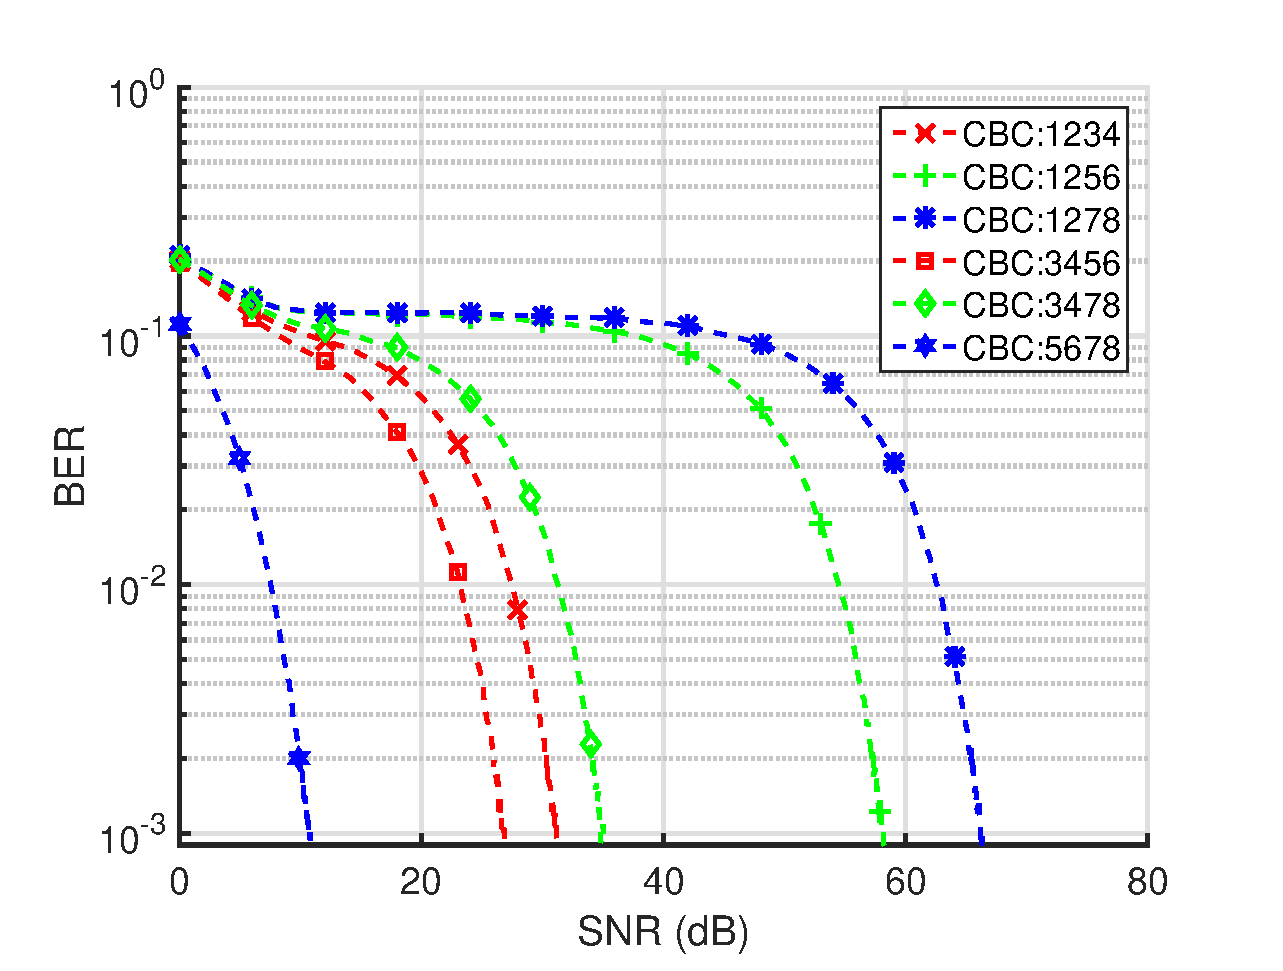
\includegraphics[trim={0.1in 0.0in 0.5in 0.1in}, clip=true, width=\textwidth]{M4_N5_4-MM_BERvsSNR.eps}
			\caption{4-MM, $D$=5}
			\label{fig4MM5}
		\end{subfigure}
		%\hfill
		\begin{subfigure}{0.49\textwidth}
		\centering
			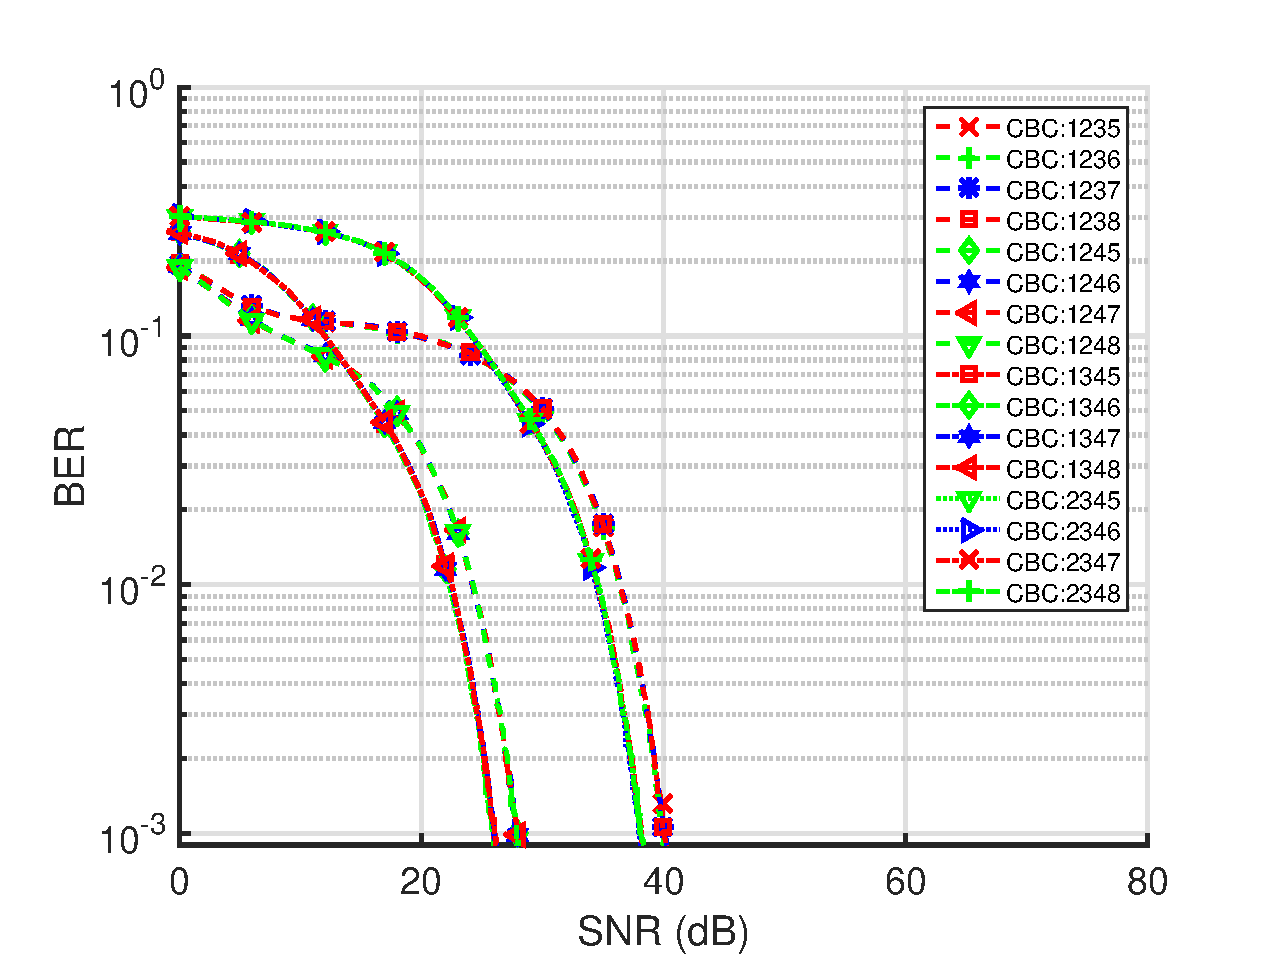
\includegraphics[trim={0.1in 0.0in 0.5in 0.1in}, clip=true, width=\textwidth]{M4_N6_4-MM_BERvsSNR.eps}
			\caption{4-MM, $D$=6}
			\label{fig4MM6}
		\end{subfigure}
		%\vfill
		\begin{subfigure}{0.49\textwidth}
		\centering
			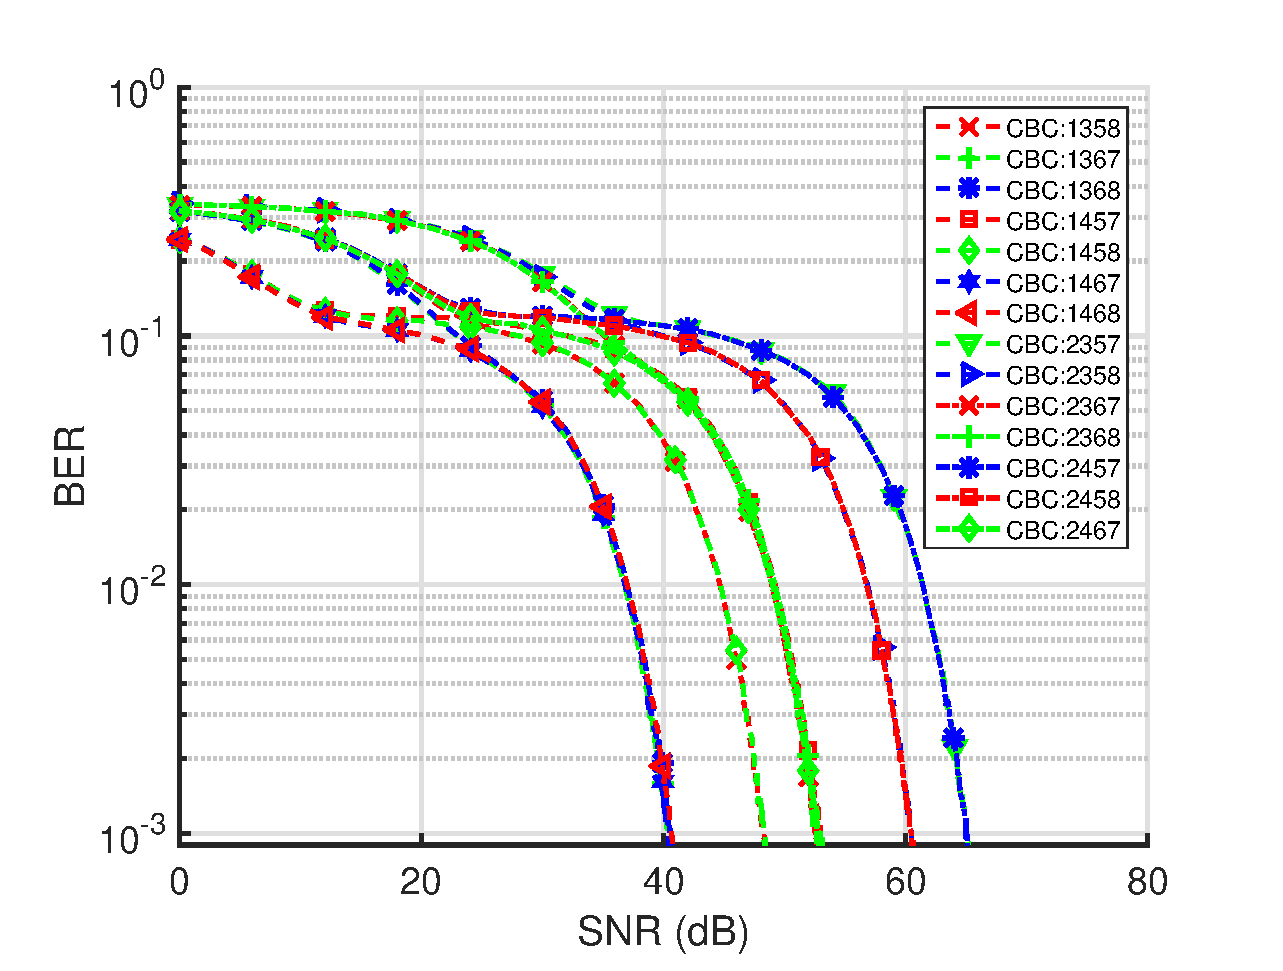
\includegraphics[trim={0.1in 0.0in 0.5in 0.1in}, clip=true, width=\textwidth]{M4_N7_4-MM_BERvsSNR.eps}
			\caption{4-MM, $D$=7}
			\label{fig4MM7}
		\end{subfigure}
		%\hfill
		\begin{subfigure}{0.49\textwidth}
		\centering
			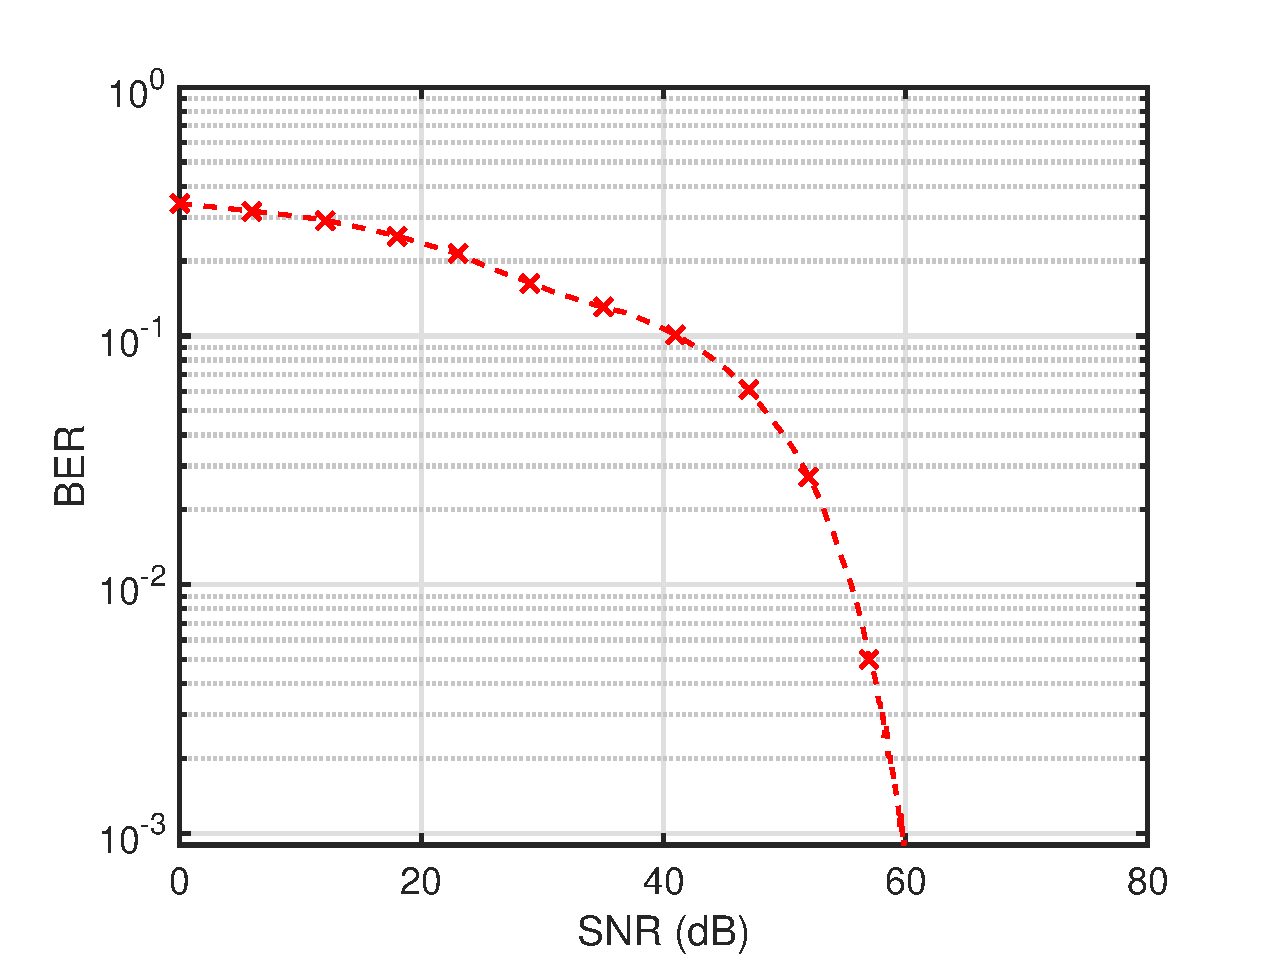
\includegraphics[trim={0.1in 0.0in 0.5in 0.1in}, clip=true, width=\textwidth]{M8_N7_8-MM_BERvsSNR.eps}
			\caption{8-MM, $D$=7}
			\label{fig8MM7}
		\end{subfigure}
	\caption{BER vs SNR for different combinations of CBC}
	\label{figMM_BERvsSNR}
\end{figure}
\end{landscape}
\clearpage% Flush page
}

Performance of metameric modulation is studied using color bands and color band combinations as defined in IEEE 802.15.7. Each set of LEDs generating a metameric color point can be implemented as a CBC. Block diagram for MM using using CBCs is illustrated in \figurename{ \ref{figMMBD}}. For an $M$-ary MM, $m=$ log$^{ }_{2}$($M$) bits from the incoming bit--stream are encoded to one out of $M$ possible CBCs. With knowledge of color set--point to generate and user requested illumination level, radiant fluxes P$_{\text{d}}; 1\leq\text{d}\leq$ D to transmit are calculated. The LED drivers then drive all LEDs to achieve desired illumination color and intensity using the CBC selected by the information to transmit. At the receivers, the incident radiant flux generates electrical signals which are used to estimate transmitted flux $\hat{\text{P}}_{\text{d}}$ over each type of LED. Using the estimated fluxes, an estimate of active set of LEDs $\hat{\text{CBC}}_{m}$ can be made to recover transmitted information. {\color{red}May need to substitute K for D.}

The IEEE 802.15.7 standard defines 7 color bands. Thus for this analysis, D=7 is considered. \figurename{ \ref{figMM_BERvsSNR}} shows BER vs SNR performance for MM. For this analysis, a white chromaticity point of (1/3, 1/3) is generated with the selected CBCs. 4-MM can be implemented with K = 5, 6 or 7. 8-MM is implemented with K = 7. In absence of illumination constraint, 4-MM achieves the best performance with K = 5 using CBs from set \{0,1,2,3,4\} for CBC set \{5,6,7,8\}. Performance plots for 4-MM with K = 6 and 7 are also illustrated for comparison. Implementing 8-MM with CBCs as outlined in IEEE 802.15.7 requires about 60 dB of SNR and seems impractical. However, a different set of LEDs may be used to implement 8-MM to obtain a better performance.

Performance comparison of 4-MM at same illumination intensity level is illustrated in \figurename{ \ref{figMM_BERvsSNR}}. In this case, with K = 5, 4-MM with CBs from set \{0,1,2,4,5\} for CBC set \{3,4,5,6\} outperforms others.  CBC set \{5,6,7,8\} has a high luminous efficacy as compared to  CBC set \{3,4,5,6\} and thus is constrained in radiant flux for signaling at a set illumination level. On comparing performance of 4-MM for all possible values of $K$, CBC sets \{1,2,4,5\}, \{1,2,4,6\}, \{1,2,4,7\} and \{1,2,4,8\} with $K$ = 6 perform the best.

\afterpage{%
\clearpage
\begin{landscape}% Landscape page
\begin{figure}[b]
	\centering
		\begin{subfigure}{0.49\textwidth}
		\centering
			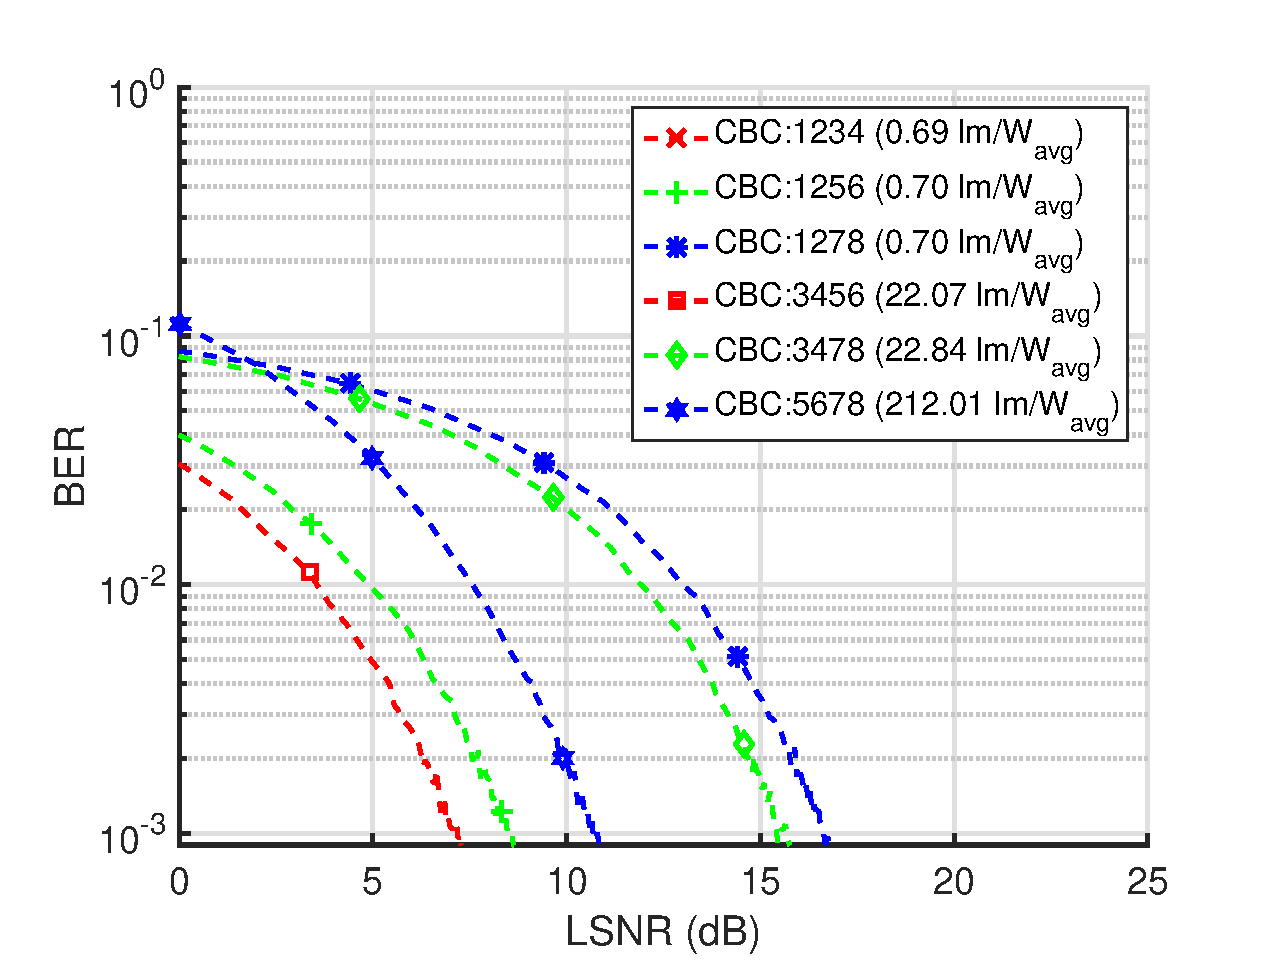
\includegraphics[trim={0.1in 0.0in 0.5in 0.1in}, clip=true, width=\textwidth]{M4_N5_4-MM_BERvsLSNR.eps}
			\caption{4-MM, $D$=5}
			\label{fig4MM5L}
		\end{subfigure}
		%\hfill
		\begin{subfigure}{0.49\textwidth}
		\centering
			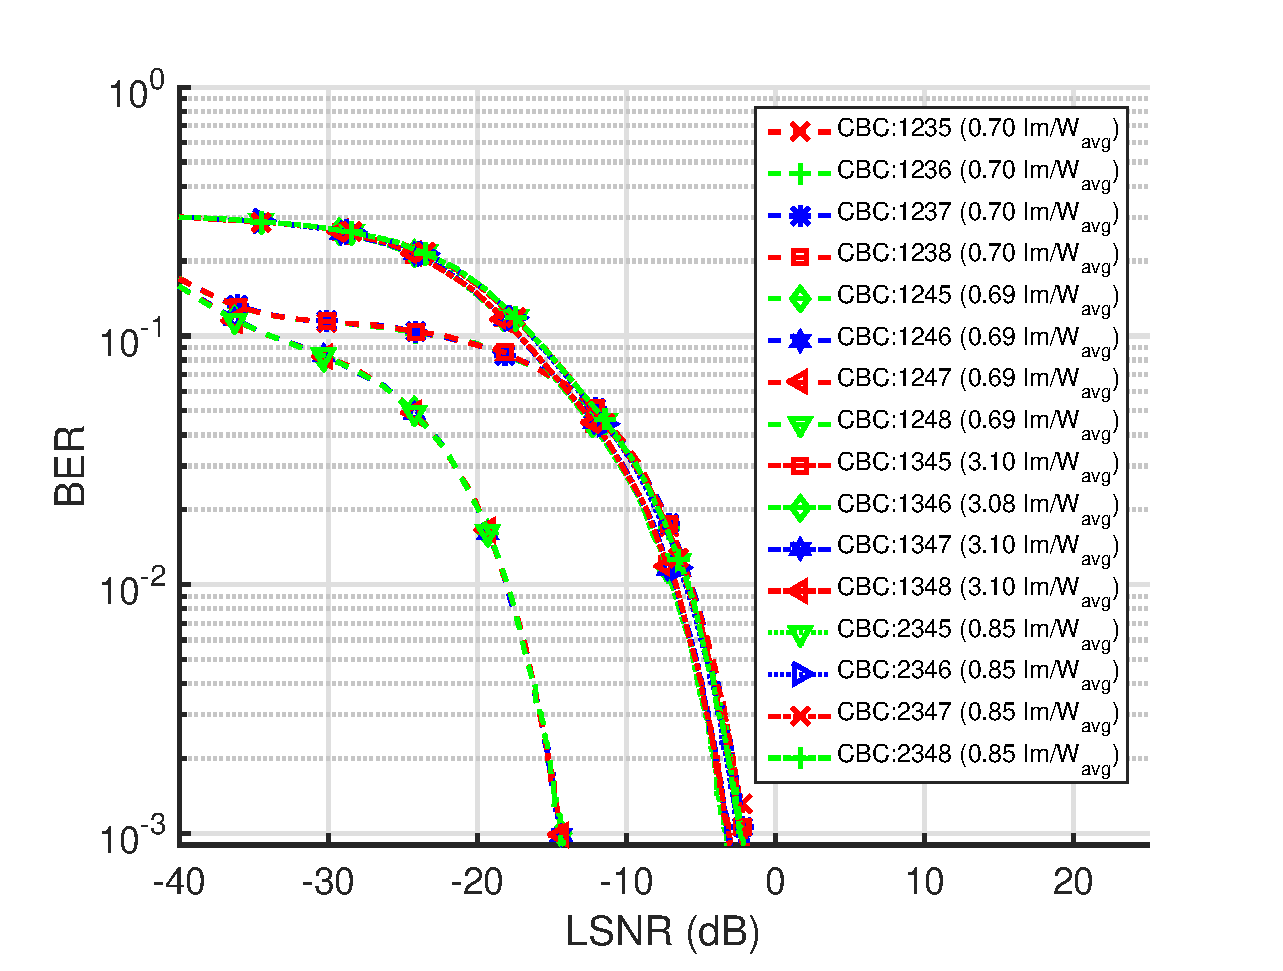
\includegraphics[trim={0.1in 0.0in 0.5in 0.1in}, clip=true, width=\textwidth]{M4_N6_4-MM_BERvsLSNR.eps}
			\caption{4-MM, $D$=6}
			\label{fig4MM6L}
		\end{subfigure}
		%\vfill
		\begin{subfigure}{0.49\textwidth}
		\centering
			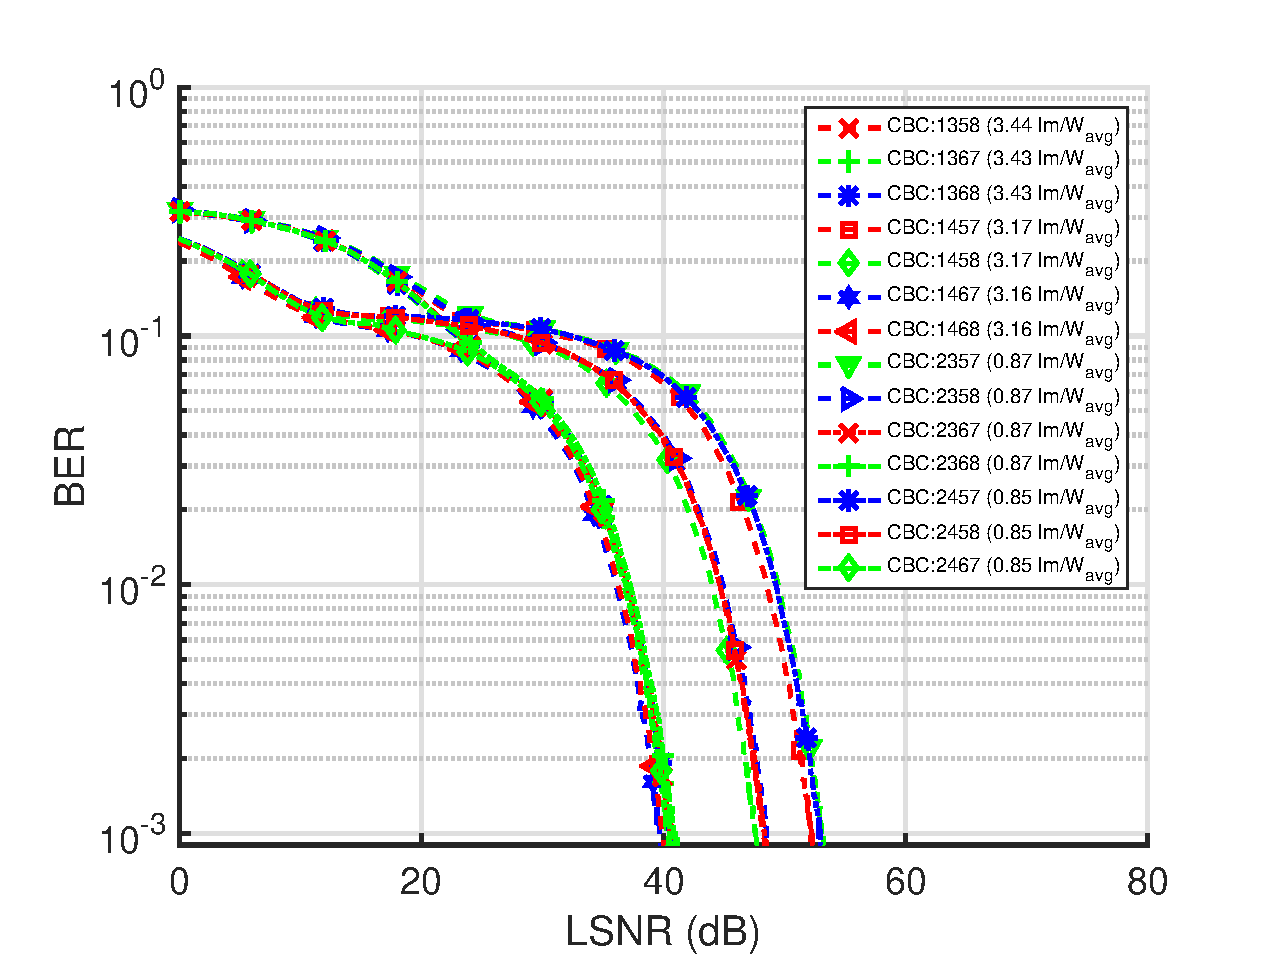
\includegraphics[trim={0.1in 0.0in 0.5in 0.1in}, clip=true, width=\textwidth]{M4_N7_4-MM_BERvsLSNR.eps}
			\caption{4-MM, $D$=7}
			\label{fig4MM7L}
		\end{subfigure}
		%\hfill
		\begin{subfigure}{0.49\textwidth}
		\centering
			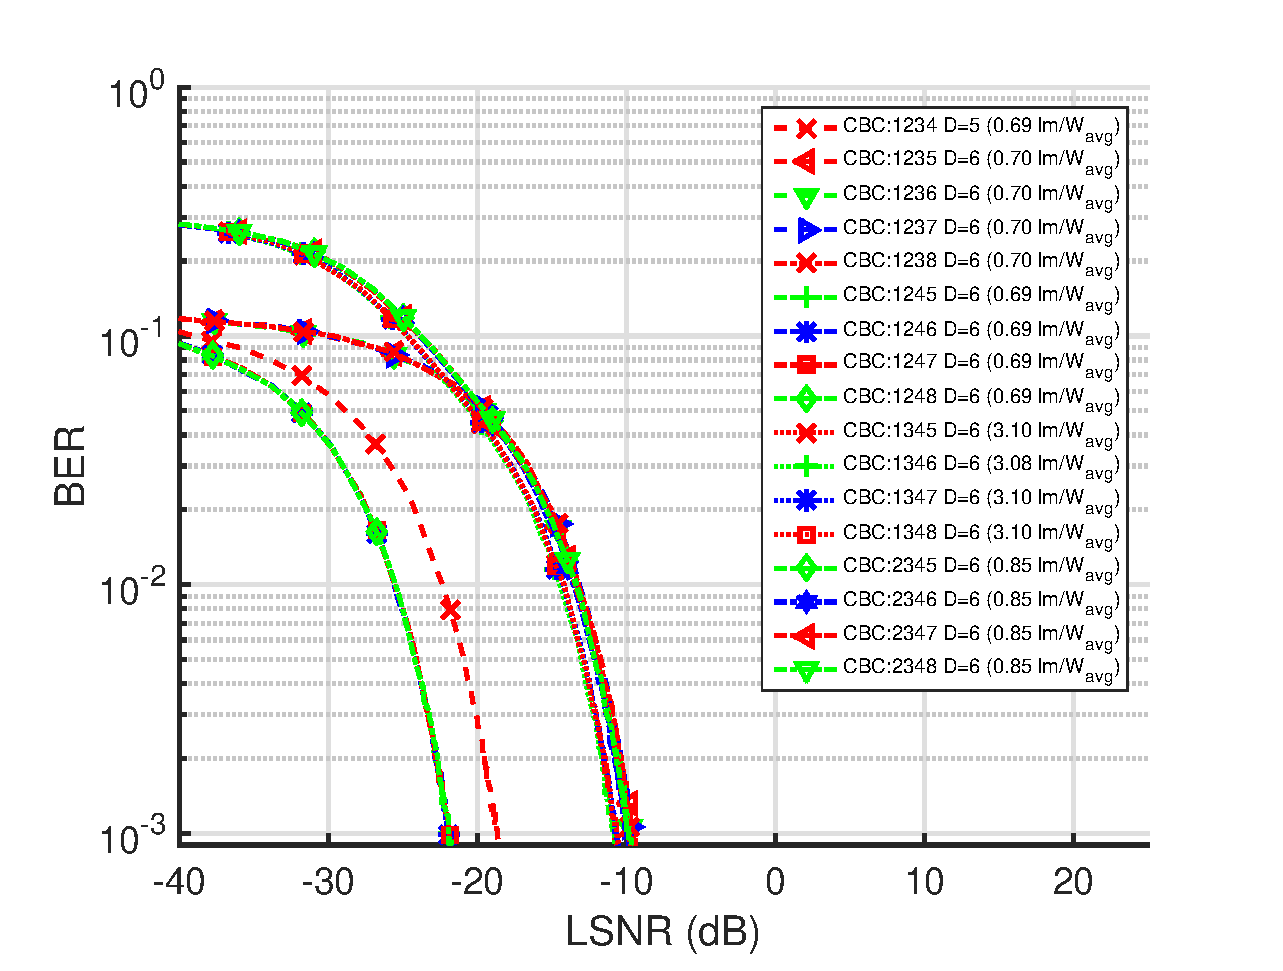
\includegraphics[trim={0.1in 0.0in 0.5in 0.1in}, clip=true, width=\textwidth]{4-MM_BERvsLSNR.eps}
			\caption{4-MM}
			\label{fig4MML}
		\end{subfigure}
	\caption{BER vs LSNR for different combinations of CBC}
	\label{figMM_BERvsLSNR}
\end{figure}
\end{landscape}
\clearpage% Flush page
}